\documentclass[slidestop,compress,mathserif, xcolor=table]{beamer}
\usetheme{Madrid}
\setbeamertemplate{headline}{}
\definecolor{scigreen}{RGB}{70,116,60}
\setbeamercolor{structure}{fg=scigreen}
\setbeamercovered{highly dynamic}

\usepackage[T1]{fontenc}
\usepackage[utf8]{inputenc}
\usepackage[english]{babel}
\usepackage{graphicx}
\usepackage{amsmath}
\usepackage{amssymb}
\usepackage{listings}

\title{Improving Rasterific}
\author[Chi, William]{Chi, William}
\institute[DIKU]{Department of Computer Science, University of Copenhagen}
\date{\today}

\begin{document}

\frame{\titlepage}
\begin{frame}[c]{Project}
    \begin{itemize}
    \item Briefly describe
    \item what this project is about
    \end{itemize}
\begin{figure}
\centering
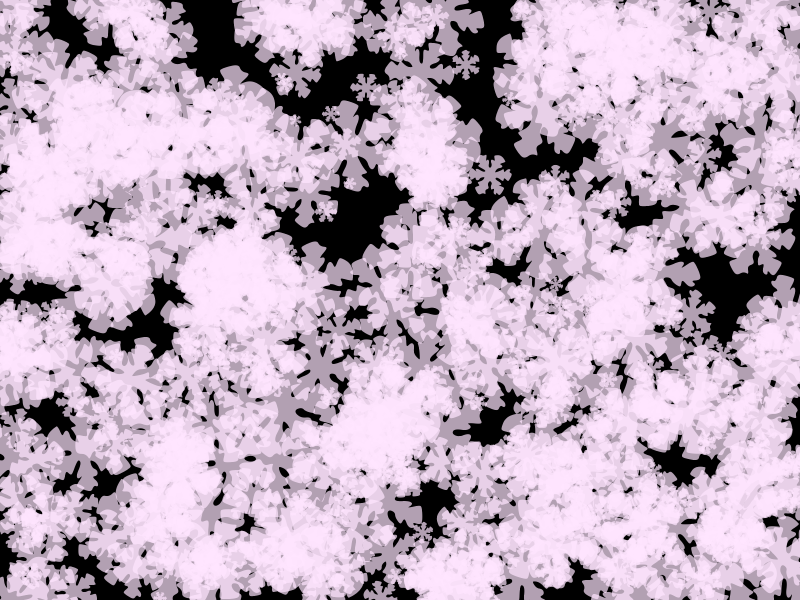
\includegraphics[width=0.3\linewidth]{../flakes}

\includegraphics[width=0.3\linewidth]{../bigsquare}
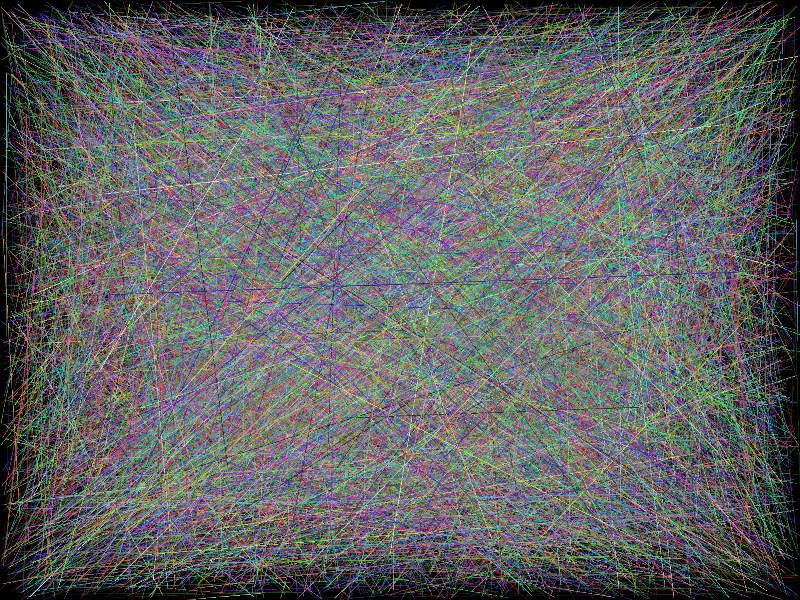
\includegraphics[width=0.3\linewidth]{../lines}
\end{figure}
\end{frame}

\begin{frame}[c]{Rasterific}
About the implementation + pipeline picture.

Maybe split in two slides
\end{frame}

\begin{frame}[c]{Experiments}
overview of experiments - use same pipeline picture, annotated (on the same position in the slide for maximum goodness)

I have an idea for a tree-like picture - TBA
\end{frame}

\begin{frame}[c]{Decomposition of \texttt{Primitives}}
description + threadscope.

NOTE: each experiment slide should be fairly brief during presentation -- not too many technical details, rather an explanation of parallel granularity + what we saw in threadscope
\end{frame}

\begin{frame}[c]{Sorting \texttt{EdgeSamples}}
description + threadscope
\end{frame}

\begin{frame}[c]{Combining \texttt{EdgeSamples}}
description + threadscope
\end{frame}

\begin{frame}[c]{Filling \texttt{DrawOrders}}
description + threadscope
\end{frame}

\begin{frame}[c]{Benchmarks and Results}
maybe some graphical representation of the table from the report
\end{frame}

\begin{frame}[c]{Evaluation}
Why we got these results
\end{frame}

\begin{frame}[c]{Further Work and Conclusion}
\end{frame}
\end{document}